\documentclass[12pt,letterpaper]{report}
\usepackage[margin=1in]{geometry}
\usepackage{graphicx}
\usepackage{amsmath}
\usepackage[font=small,labelfont=bf]{caption}
\usepackage[justification=centering]{caption}
\usepackage{tikz}
\usepackage{circuitikz}
\usepackage{siunitx}
\usepackage{float}
\newlength \figwidth
\setlength \figwidth {0.75\linewidth}
\newcommand{\parallelsum}{\mathbin{\|}}

\begin{document}

\title{E153 Laboratory Assignment \#7}
\author{Courtney Keeler and Stephen Pinto\\
Harvey Mudd College}
\date{November 20, 2013}
\maketitle

\section*{List of Materials}
\begin{itemize}
	\item Tektronix 2212 Oscilloscope
	\item Pomona 4550B (10X probe)
	\item Elenco LCM-1950 Multimeter
	\item 2N3904 transistor (NPN)
	\item 2N3906 transistor (PNP)
	\item Standard resistors
	\item Standard capacitors
\end{itemize}

\section*{Purpose}
The purpose of this lab is to explore the Complementary Push Pull Amplifier by building one designed in class to compare with simulations, adding the Push Pull to the Common Emitter Amplifier from lab 6 to compare the results with the single emitter follower.

\section*{Push Pull Amplifier}

\begin{figure}[H]
\centering
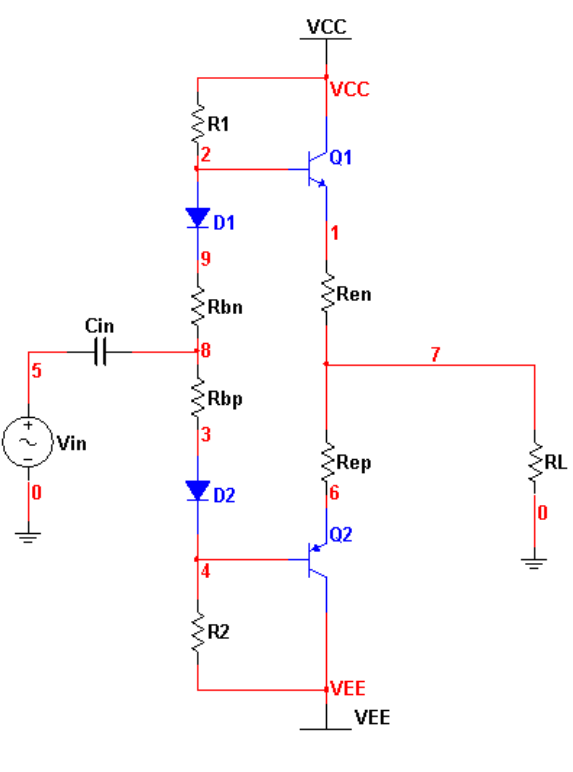
\includegraphics[width=\figwidth, keepaspectratio=true]{lab7_images/push_pull.png}
\caption{Class AB Push Pull Follower. Image from Lecture 12.}
\label{fig:push_pull}
\end{figure}

\subsection*{Procedure}

\begin{enumerate}
\item Measure the actual component values used in the Push Pull design (shown in Fig. \ref{fig:push_pull})
\item Build the Complementary Push Pull Amplifier with the measured components
\item Compare the actual gain and frequency response values with the simulated values
\end{enumerate}

\subsection*{Calculations \& Expectations}

Measured component values for the constructed complementary push pull amplifier are:
\begin{itemize}
\item $R_1$ = 14.65 k$\Omega$
\item $R_{bn}$ = 15 $\Omega$
\item $R_{en}$ = 118 $\Omega$

\item $R_2$ = 14.76 k$\Omega$
\item $R_{bp}$ = 15 $\Omega$
\item $R_{ep}$ = 118 $\Omega$

\item $R_L$ = 981 $\Omega$
\item $\beta_{1}$ = 183
\end{itemize}

In this lab we will be loading the Common Emitter Amplifier (CEA) from lab 6 with the complementary push pull amplifier. Due to the loading effect, there should be some attenuation on the AC output from the CEA equal to

$$
A = \frac{R_{in,PPA}}{R_{in,PPA} + R_{out,CEA}}
$$

where $R_{in,PPA}$ is the input resistance of the push pull amplifier. As derived in class, this input resistance is

$$
R_{in,PPA} = R_1 \parallelsum R_2 \parallelsum (r_{\pi} + (1 + \beta)(R_e + R_L)) = 7.1 k\Omega.
$$

The above calculated value for $R_{in,PPF}$ assumes that $r_{\pi} \ll (1 + \beta)(R_e + R_L)$ - which is reasonable given the values of $\beta_1$, $R_e$, and $R_L$. $R_out$ of the Common Emitter Amplifier from lab 6 is about 18 $k\Omega$, making the expected attenuation to be roughly 0.3.

As for the output from the push pull amplifier, the expected gain of the system, as derived in class, is

$$
A_v = \frac{R_L}{R_E  + R_L} = 0.9.
$$


\subsection*{Results}



\section*{Conclusion}

In conclusion, we have demonstrated expected functionality of the complementary push pull amplifier in two ways. Firstly, we have confirmed its input resistance by demonstrating attenuation due to loading by cascading it with the Common Emitter Amplifier from lab 6, of which we know the output resistance. Secondly, we have confirmed its gain by measuring the magnitude of the input and output AC signal. In both cases, our measured results were within 10\% of expected, an error margin attributable to simplifying assumptions and measurement error. We were able to listen to our output signal on speakers and hear the tone and volume change as we varied frequency and amplitude, though the sound was very weak in all cases.

The performance of this push pull follower is sub-par compared to that of the simple emitter follower from lab 6 only because we did not design this push pull amplifier to be in cascade with the CEA. Meaning their input and output resistances of the PPA and CEA respectively are incorrectly proportioned such that there is an unreasonable amount of attentuation between the two stages. However, this push pull amplifier wastes much less power than the simple emitter follower. Were it designed correctly, the efficiency of the push pull amplifier would make it a superior choice in most cases.

\end{document}

%photo 297: output of entire CE circuit, shows gain at 25 Hz
%photo 298: voltage after stage 1
%photo 299: voltage after emitter follower (it's been shifter down by 0.7!)

%\begin{table}[ht]
%\caption{Voltage across each "diode"} % title of Table
%\centering 
%    \begin{tabular}{| c | c |} 
%    \hline
%    $V_{\text{BC}}$ & 0.711 V \\
%    $V_{\text{BE}}$ & 0.717 V \\
%    \hline
%    \end{tabular}
%    \label{table:section_1}
%\end{table}

%input=500mvpp, 1kHz freq, high Z
%changing R1 of the CE amp to 15Mohm to try to lower the dc offset of output. new offset of output is 14.11 V (just within the +/- 5V requirement)
%output gain of CE: 4.741 V amplitude which means 10.22 Vpp (recall for 400 mV in)
%
%now we're changing R1 to 10K and R2 is 12K for now, may increase

%nevermind, we don't need to change the CE amp. We just have the consider the massive output impedance of the CE interfacing with the smaller input impedance of the push pull.
%
%photo 325: uncoupled output
%photo 326: coupled output (output from CE with a load)
%photo 327: DC offset CE amp output
%photo 328: push pull output (notice no DC offset!, but massive attenuation)

%npn beta is 183
